\documentclass[10.5pt]{article}
\usepackage{a4wide}
%\usepackage[cm]{fullpage} si lo queremos mas ancho

\usepackage[backend=biber, style=numeric, uniquename=false]{biblatex}
%style=authoryear

\usepackage[spanish,activeacute]{babel}
\usepackage[utf8]{inputenc}
\usepackage{enumerate}
\usepackage{todonotes}
\usepackage{listings}
\usepackage{verbatim}
\usepackage{stmaryrd}
\usepackage{amsmath}
\usepackage{systeme}


\begin{document}
\date{Mayo de 2016}
\title{Ecuaciones Diferenciales y\\Métodos Numéricos Aplicados\\Trabajo Práctico}
\author{Manuel F. Martín}

\maketitle


\section*{Parte A}

\begin{enumerate}
 
 \item Para escribir la función de la deformada, partimos del dato de que sigue una deformación cosenoidal y,
a partir de la representación gráfica y la ubicación de los ejes, notamos que está desplazada en sentido vertical.

Luego de ésto planteamos la forma general del coseno \[U_g(x) = A \cos (px) + n\]

Como dato sabemos que la amplitud del coseno es
$\Delta_{max}$, por lo tanto el desplazamiento es $\frac{\Delta_{max}}{2}$. Basándonos en esta información reemplazamos el $n$ por
$\frac{\Delta_{max}}{2}$, obteniendo \[U_g(x) = A \cos (px) + \frac{\Delta_{max}}{2}\]

Después de ésto, utilizamos las condiciones de contorno en $x = 0$ y $ x = L$, con las cuales obtenemos el valor de las constantes
$A$ y $p$, para completar así la función de la deformada.

\[U_g(0) = A \cos (p0) + \frac{\Delta_{max}}{2} = 0 \Rightarrow A = -\frac{\Delta_{max}}{2}\]
\[U_g(L) = -\frac{\Delta_{max}}{2} \cos (pL) + \frac{\Delta_{max}}{2} = 0 \Rightarrow \cos (pL) = 1 \Rightarrow pL = 0 \vee pL = 2\pi\]

Pero $pL$ no puede ser $0$, ya que por dato sabemos que $L$ es $12m$, la longitud del tramo del puente,
mientras que $p$ no puede ser $0$ porque si así lo fuese, $\cos(px)$ siempre sería $0$. Entonces,

\[ pL = 2\pi \Rightarrow p = \frac{2\pi}{12} \Rightarrow p = \frac{\pi}{6} \]

Por lo tanto, la función de la deformada es 

\[U_g(x) = -\frac{\Delta_{max}}{2}  \cos (\frac{\pi}{6}x) + \frac{\Delta_{max}}{2} \]

 \item Para obtener la ley de la deformada en función del tiempo, nos basamos en la función obtenida en el apartado anterior.
Sabemos que la velocidad es el cociente entre la distancia y el tiempo, es decir, $x = v \times t$. Luego, para escribir la deformada
en función del tiempo, debemos sustituir $x$ por $v \times t$, ya que en el eje $x$ tenemos un moviento rectilíneo uniforme.
Entonces, la función obtenida, depende de $v \times t$. Sin embargo, al ser $v$ constante, sale de los argumentos de la función,
obteniendo de esta manera la función de la deformada en función de $t$.

\[U_g(t) = -\frac{\Delta_{max}}{2}  \cos (\frac{\pi v}{6}t) + \frac{\Delta_{max}}{2} \]

 \item Esta ecuación diferencial es de tipo ordinaria, ya que sólo tiene una variable 
independiente que es el tiempo. También es de segundo orden, ya que la derivada de mayor
grado presente es una derivada segunda.
Además podemos decir que es una EDO lineal no homogénea a coeficientes constantes. Primero es de tipo lineal dado que las derivadas están
acompañadas de coeficientes constantes, ya que éstos no varían en función del tiempo. Por otro lado, decimos que es de tipo no homogénea,
debido a que está igualada a una función no nula.

 \item Los métodos numéricos que podemos utilizar para resolver este problema son Euler, Heun
y Runge Kutta, dado que el mismo está planteado mediante una ecuación diferencial, y estos
métodos son los apropiados para este tipo de ecuaciones.

Sin embargo no lo podemos resolver en forma directa, ya que nuestra ecuación diferencial es de segundo orden, y los métodos
mencionados sirven para resolver ecuaciones diferenciales de primer orden solamente. Debido a ésto, debemos reescribir la ecuación
transformándola en una de primer orden, y formando de esta manera un sistema de ecuaciones de primer orden, el cual es equivalente a la
ecuación de segundo orden original.

Para hacer ésto, definimos la función $T$, tal que $T(t) = \dot U(t)$. Luego, $\dot T(t) = \ddot U(t)$.

%\systeme*{m \dot T(t) + c T(t) + k U(t) = -m \ddot U_g(t), \dot T(t) = \ddot U(t)}
\[
\begin{cases}
  &m \dot T(t) + c T(t) + k U(t) = -m \ddot U_g(t) \\
  &\dot T(t) = \ddot U(t)
\end{cases}
\]

En mi opinión, el método de Runge Kutta de orden cuatro es el más indicado, ya que nos entrega un resultado más preciso que Euler y Heun, 
y a pesar de que el gasto computacional es más elevado que en el resto de los casos, no es tan grande, y de esta forma, obtenemos un resultado
más cercano al real.

 \item Las condiciones que requerimos para poder resolver esta ecuación diferencial son dos.
La primera es que la posición vertical $U(t)$, para el tiempo $0$ es $0$, es decir, $U(0) = 0$, y la segunda es que
la velocidad vertical para el tiempo $0$ es $0$, ya que el auto viene desplazándose en una
superficie plana, por lo tanto en ese instante no tiene velocidad vertical, lo que notamos $\dot U(0) = 0$.

 \item Pseudocódigo para obtener la historia del desplazamiento vertical relativo.
 \begin{verbatim}
m = masa
k = rigidez del resorte
c = constante del amortiguador
dMax = deformación máxima
v = velocidad del automóvil
cantTramos = cantidad de tramos del puente
 
La función d2Ug es la derivada segunda de la función que calcula la deformada.
La definimos para usarla al momento de calcular la pendiente.
FUNCION d2Ug(t) 
    extra = pi/6 * v
    DEVUELVE dMax/2 * extra^2 * cos(t * extra)

X0 = (condición inicial para U, condición inicial para T)

La función f calcula la pendiente necesaria para usar el método RK.
Dependiendo de la posición del auto, debemos usar un movimiento forzado
amortiguado o un movimiento libre amortiguado.
La variable X es un par que contiene los dos valores obtenidos en la
iteración anterior.
FUNCION f(t, Xi)
    Xi+1(1) = Xi(2)
    SI v*t <= cantTramos * longTramos ENTONCES
        Xi+1(2) = -(m * d2Ug(t, v) + c * Xi(2) + k * Xi(1))/m
    SI NO Xi+1(2) = -(c * Xi(2) + k * Xi(1))/m
    DEVUELVE Xi+1

ti = tiempo inicial
tf = tiempo final
paso = paso de tiempo

LLAMA al método encargado de calcular RK, pasándole la información y las funciones
definidas previamente.
\end{verbatim}

\end{enumerate}


\section*{Parte B}

\begin{enumerate}

\item Ver \textbf{Anexo: Scilab}.

\begin{enumerate}
  \item \text{} \\
  \centerline{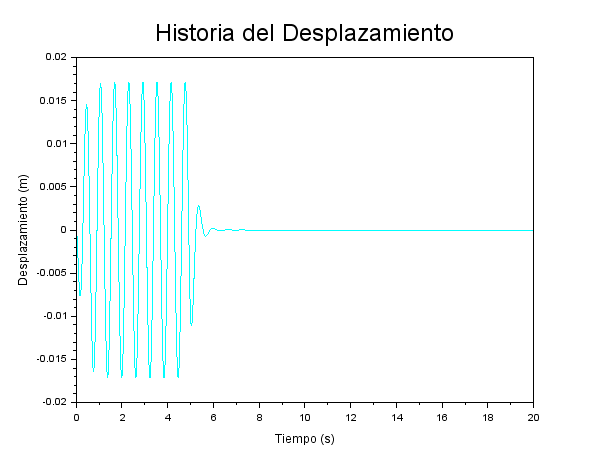
\includegraphics[width=15cm]{graf1}}
  \item  El valor máximo del desplazamiento para una velocidad de $70Km/h$ y un paso de $0.001s$ es $0.0171204m$.
\end{enumerate}
 
 \item Ver \textbf{Anexo: Scilab}. \\
  \centerline{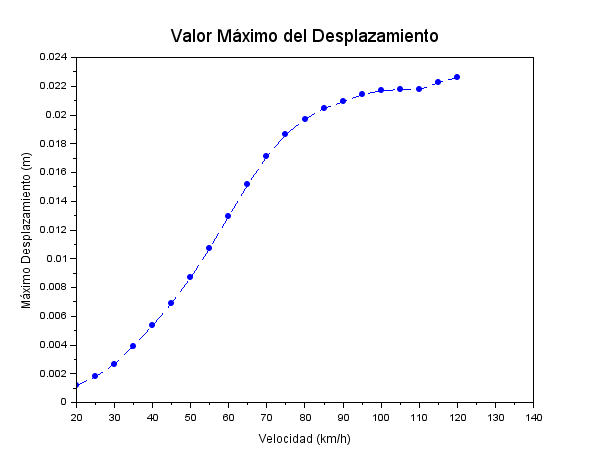
\includegraphics[width=15cm]{graf2}}
  
 \item Con respecto a este problema en particular podemos concluir que la velocidad con que ingresa el vehículo al puente influye de
 manera directa en el desplazamiento vertical que sufre el móvil mientras transita sobre el mismo. Cuanto mayor sea la velocidad, más grande
 va a ser el desplazamiento. Además de ésto, la velocidad también afecta el tiempo que tarda en desaparecer el movimiento vertical, a menor
 velocidad más rápido se estabiliza el vehículo.
 
 En ingeniería utilizamos frecuentemente EDOs para representar y predecir situaciones físicas reales. Dado ésto, muchas veces necesitamos
 resolver esas EDOs para poder calcular la información que necesitamos, pero nos encontramos con que las soluciones exactas no están disponibles
 o son muy difíciles de obtener. Es aquí donde recurrimos al uso de métodos numéricos, que si bien no nos devuelven el valor exacto, nos brindan
 la posibiladad de obtener una solución aproximada, la cual nos permite resolver problemas reales.
 
 Si bien los métodos numéricos están disponibles desde hace mucho tiempo, hasta no hace tanto su uso era casi imposible ya que los cálculos debían
 realizarse manualmente, llevando muchísimo tiempo y generando una gran posibilidad de equivocarse. Los avances tecnológicos han hecho posible la
 difusión de estos métodos, ya que hoy en día podemos aplicarlos de manera sencilla utilizando computadoras standard. 
 \end{enumerate}

\newpage
\section*{Anexo: Scilab}

\verbatiminput{TP.sce}

\end{document}
